% This is the Reed College LaTeX thesis template. Most of the work
% template. Later comments etc. by Ben Salzberg (BTS). Additional
% restructuring and APA support by Jess Youngberg (JY).
% Your comments and suggestions are more than welcome; please email
% them to cus@reed.edu
%
% See http://web.reed.edu/cis/help/latex.html for help. There are a
% great bunch of help pages there, with notes on
% getting started, bibtex, etc. Go there and read it if you're not
% already familiar with LaTeX.
%
% Any line that starts with a percent symbol is a comment.
% They won't show up in the document, and are useful for notes
% to yourself and explaining commands.
% Commenting also removes a line from the document;
% very handy for troubleshooting problems. -BTS

% As far as I know, this follows the requirements laid out in
% the 2002-2003 Senior Handbook. Ask a librarian to check the
% document before binding. -SN

%%
%% Preamble
%%
% \documentclass{<something>} must begin each LaTeX document
\documentclass[12pt,twoside]{reedthesis}
% Packages are extensions to the basic LaTeX functions. Whatever you
% want to typeset, there is probably a package out there for it.
% Chemistry (chemtex), screenplays, you name it.
% Check out CTAN to see: http://www.ctan.org/
%%
\usepackage{graphicx,latexsym}
\usepackage{amsmath}
\usepackage{amssymb,amsthm}
\usepackage{longtable,booktabs,setspace}
\usepackage{chemarr} %% Useful for one reaction arrow, useless if you're not a chem major
\usepackage{rotating}

% Modified by CII
\usepackage[hyphens]{url}
\usepackage{hyperref}
\usepackage{lmodern}

% Added by CII (Thanks, Hadley!)
% Use ref for internal links
\renewcommand{\hyperref}[2][???]{\autoref{#1}}
\def\chapterautorefname{Chapter}
\def\sectionautorefname{Section}
\def\subsectionautorefname{Subsection}

\usepackage{caption}
\captionsetup{width=5in}

% \usepackage{times} % other fonts are available like times, bookman, charter, palatino

\title{Political Ideology and Congressional Leadership}
\author{Hans Trautlein}
% The month and year that you submit your FINAL draft TO THE LIBRARY (May or December)
\date{May 2016}
\division{History and Social Sciences}
\advisor{Alexander H. Montgomery}
%If you have two advisors for some reason, you can use the following
\altadvisor{}
%%% Remember to use the correct department!
\department{Political Science}
% if you're writing a thesis in an interdisciplinary major,
% uncomment the line below and change the text as appropriate.
% check the Senior Handbook if unsure.
%\thedivisionof{The Established Interdisciplinary Committee for}
% if you want the approval page to say "Approved for the Committee",
% uncomment the next line
%\approvedforthe{Committee}

% Below added by CII

%%% Copied from knitr
%% maxwidth is the original width if it's less than linewidth
%% otherwise use linewidth (to make sure the graphics do not exceed the margin)
\makeatletter
\def\maxwidth{ %
  \ifdim\Gin@nat@width>\linewidth
    \linewidth
  \else
    \Gin@nat@width
  \fi
}
\makeatother

\renewcommand{\contentsname}{Table of Contents}

\setlength{\parskip}{0pt}


\providecommand{\tightlist}{%
  \setlength{\itemsep}{0pt}\setlength{\parskip}{0pt}}

\Acknowledgements{

}

\Dedication{

}

\Preface{

}

\Abstract{
This paper examines the differences in ideology in Congress between
non-leaders and congressional leaders, the speakers, and whips. While
past research has looked at the ideology of congressional leaders before
they have taken their positions of power they have neglected to look at
how their ideology changes as they have taken to their new position
within the congressional power structure. Using measures of ideology
from a \texttt{NOMINATE} dataset we fit models based on party and
leadership status. The leaders are then compared to the non-leaders on
how their ideology changes compared to the mean ideology of Congress at
the time and the models are assessed for statistical significance.
Results are then expanded on and a discussion follows.
}

\usepackage{setspace}

%%
%% End Preamble
%%
%

\begin{document}

      \maketitle
  
  \frontmatter % this stuff will be roman-numbered
  \pagestyle{empty} % this removes page numbers from the frontmatter

  
  
  % Add table of abbreviations?

      \hypersetup{linkcolor=black}
    \setcounter{tocdepth}{2}
    \tableofcontents
  
      \listoftables
  
      \listoffigures
  
      \begin{abstract}
      This paper examines the differences in ideology in Congress between
      non-leaders and congressional leaders, the speakers, and whips. While
      past research has looked at the ideology of congressional leaders before
      they have taken their positions of power they have neglected to look at
      how their ideology changes as they have taken to their new position
      within the congressional power structure. Using measures of ideology
      from a \texttt{NOMINATE} dataset we fit models based on party and
      leadership status. The leaders are then compared to the non-leaders on
      how their ideology changes compared to the mean ideology of Congress at
      the time and the models are assessed for statistical significance.
      Results are then expanded on and a discussion follows.
    \end{abstract}
  
  
  \mainmatter % here the regular arabic numbering starts
  \pagestyle{fancyplain} % turns page numbering back on

  \doublespacing
  
  \begin{Shaded}
  \begin{Highlighting}[]
  \KeywordTok{source}\NormalTok{(}\StringTok{'~/thesis/rcode/plot_ideas.R'}\NormalTok{, }\DataTypeTok{echo=}\OtherTok{FALSE}\NormalTok{)}
  \end{Highlighting}
  \end{Shaded}
  
  \begin{verbatim}
  
  Attaching package: 'dplyr'
  \end{verbatim}
  
  \begin{verbatim}
  The following objects are masked from 'package:stats':
  
      filter, lag
  \end{verbatim}
  
  \begin{verbatim}
  The following objects are masked from 'package:base':
  
      intersect, setdiff, setequal, union
  \end{verbatim}
  
  \chapter*{Introduction}\label{introduction}
  \addcontentsline{toc}{chapter}{Introduction}
  
  This paper examines the differences in ideology in Congress between
  non-leaders and congressional leaders, the speakers, and whips. While
  past research has looked at the ideology of congressional leaders before
  they have taken their positions of power they have neglected to look at
  how their ideology changes as they have taken to their new position
  within the congressional power structure. Using measures of ideology
  from a \texttt{NOMINATE} dataset we fit models based on party and
  leadership status. The leaders are then compared to the non-leaders on
  how their ideology changes compared to the mean ideology of Congress at
  the time and the models are assessed for statistical significance.
  
  \chapter{Literature Review}\label{literature-review}
  
  \section{Congressional Leaders}\label{congressional-leaders}
  
  Party leaders are hugely important in Congress. Perhaps their most
  important role is setting the legislative agenda in Congress (Rohde
  1991, @Sinclair1983). By setting the agenda in arguably the most
  powerful branch of government, congressional leaders have extraordinary
  power over which bills are brought to a vote and eventually passed. They
  also have the power of being able to shift congressional actions away
  from an otherwise sipmles answer to a problem.\footnote{For a recent
    example of this, see how in 2008 Harry Reid (D) then the majority
    leader of the Senate, was able to remove the possibility of a nuclear
    waste repository from being created at Yucca Mountain.} Leaders in
  Congress have large sway over the leaders who they can choose to fill
  the many roles below them. They are also the ``brand image'' of their
  party, especially when their party does not control the presidency.
  Understanding the ideology of leaders is important for a Congressional
  scholar to better understand why leaders act the way the do.
  
  There has often been the question of whether or not congressional
  leaders are moderates in their party, near to their party's mean, or
  extremists. Moderates would often be effective legislators, as they
  would be able to propose more centrist policies that might apply to both
  political parties. Extremists might be selected due to their ability to
  placate the louder wings of both the Republican and Democratic parties.
  A political scientist or an economist might be quick to answer that a
  congressperson near the median voter in a political party has a strong
  theoretical reasoning for being chosen. This is because votes for
  congressional leaders are votes taken solely within the party.\footnote{With
    the exception of the vote for Speaker in the House of Representatives,
    although that vote often ends up being made up entirely of the
    majority party's congresspersons voting in affirmation with the
    minority party avoiding casting a positive ballot.} The median voter
  theorem states that ``a majority rule voting system will select the
  outcome most preferred by the median voter'' (Holcombe 2006, 115). This
  builds off the assumption that there is only one dimension along which
  politics exists, for example, left to right or liberal to conservative.
  Is it also assumed that a voter will choose the option, or in this
  circumstance the politician, closest to their own ideal point along the
  singular dimension. In a majoritarian system this ideal median point
  will prevail, having more than 50\% of the vote in the final vote
  tallied.
  
  Studies have examined where leaders come from ideologically speaking.
  One has found, using the DW-NOMINATE scores of congressional leaders,
  that these leaders do in fact come from near the median of their party,
  with a tiny preference towards the slightly more extreme candidate,
  left-leaning for Democrats and right-leaning for Republicans.
  DW-NOMINATE scores place congresspersons on a single dimension from -1
  to 1, with -1 being left-leaning and 1 being right-leaning. The numbers
  are found by taking the roll call votes over a single Congress and then
  placing the legislator's scores within the range of possible values. A
  senator like Ted Cruz would end up with a number close to 1\footnote{In
    the 113th Congress his point was measured at 0.754.} whereas for
  senator like Elizabeth Warren you would see a point near to -1\footnote{In
    the 113th Congress her point was measured at -0.538}. House Democrats
  were found to be on average -0.050 away from the median point whereas
  their leaders were on overage -0.097, slightly farther away but still
  close to the median. For Senate Democrats these numbers are 0.016 and
  -0.059 respectively, again the the leaders being slighly more extreme
  than the median but still being quite close to it. For the Republicans
  the results are similar, although in the other direction. In the House,
  for leaders the average distance away from the party median for leaders
  is 0.044 whereas for the rest of the House Republicans it is -0.025. For
  the Senate Republicans the numbers are 0.048 and 0.057,
  respectively.\footnote{The Republicans in the Senate are the only group
    who elect leaders slightly more moderate on average than the party
    median in that chamber.} They find it ``hearening to note that
  leaders--who some political observers argue have strong influence over
  angenda setting and lawmaking under certain conditions--are, on balance,
  fairly representative of their parties. If leaders came from the far
  extremes of the chambers\ldots{}then policy might be even less
  reflective of the preferences of the median voter in the electorate''
  (Jessee and Malhotra 2010, see specifically 386). Jessee and Malhotra
  (2010) also find that the winner of a congressional leadership race is
  not ``ideologically distinctive'' from the entire pool candidates (2010,
  361).
  
  This evidence found in Jessee and Malhotra (2010) looked to revise
  earlier studies on the subject. Harris and Nelson (2008) looked at the
  old ``Austin-Boston'' alliance that encourage the selection of middlemen
  in the Democratic party, and also examine the changes within the
  Republican party leadership as well. Surprised by the election of the
  relatively extreme Pelosi to the Speakership, the two authors felt the
  need to revisit the question of whether the median voter theorem still
  held.\footnote{While the middle\emph{men} theory could still hold, the
    middle\emph{person} theory was in doubt.} Using the same dataset as
  Jessee and Malhotra (2010), they came to a new conclusion, that perhaps
  more partisan leaders were need as political polarization increased.
  Seeing the role switch from a place for compromise during a ``bargaining
  era and bipartisan Congress'' to a new bully pulpit, often active in the
  media and courting donors, middlepersons seemed to no longer be the most
  appropriate leaders of their party on the national stage of Congress
  (Harris and Nelson 2008, 54). Their final hypothesis is that as partisan
  divisions increase it will exacerbate the extremism of congressional
  leaders.
  
  Older research is more theoretical and is less likely to use datasets,
  like the many NOMINATE datasets available. In May (1973) leaders are
  suggested to be more extreme than the rest of their party when ideology
  is strongly important, which may connect well to the modern era. Studies
  of both British and Norwegian legislative systems cast doubt on May's
  concept, the law of curvilinear disparity.\footnote{,,todo - Unlikely
    that I should go into more depth, but maybe I could within a footnote?}
  The middleman theory is further promoted by Clausen and Wilcox (1987),
  who finds the best support for the theory in the House and then best
  within the Democratic party, which had at the time been the majority
  power for 32 years. Quickly stated, they claim that ``leaders are chosen
  who are\ldots{}dedicated to represent and prosecute the party position''
  (Clausen and Wilcox 1987, 261). More studies find evidence that leaders
  are more extreme than the median voter theorem would suggest, as
  Grofman, Koetzle, and McGann find that Democratic leaders are to the
  left of the median of their party and Republican leaders are to the
  right of the median of their party (Grofman, Koetzle, and McGann
  (2002)).
  
  \section{DW-NOMINATE}\label{dw-nominate}
  
  Keith Poole's and Howard Rosenthal's previous work about congressional
  ideology is the backbone of this study. they have constructed a way to
  fit members of Congress across a unidimensional metric that measures
  primarily ideology. Their typical dataset measures a single ``ideal
  point'' for each congressperson throughout their career and is able to
  plot them against other members of Congress throughout its existence.
  There are alternative versions of their dataset that also exist, and I
  use the Nokken and Poole version, which allows members to shift their
  ideology throughout different sessions of Congress (Nokken and Poole
  2004). There is often a clamoring by many for the structure of Congress
  to be displayed in multiple different dimesions, sometimes even one
  dimension for every issue available. More often however there is a
  request for a second dimension that allows not just a conservative
  versus liberal axis but instead a socially liberal versus socially
  conservative axis and a fiscally liberal versus fiscally conservative
  axis. While at times a second axis is useful, and in the most recent
  session of Congress can be viewed as a measure of establishment versus
  non-establishment leanings, Poole and Rosenthal as well as those who
  have use their datasets in the past primarily look to create their
  models solely from this one dimension due to its explanatory power
  (Poole and Rosenthal 2007, 21). Part of the reason why complicated
  legislators are able to represented along a single metric is due to the
  prevalence of logrolling or vote trading (Poole and Rosenthal 2007, 17).
  The primary dimension is not solely concerned with political party
  however, it also strongly relates to issues of economic redistribution
  (Poole and Rosenthal 2007, 70).
  
  Looking ahead to how the legislators, specifically the leaders, might
  change within my own study is evidence that ``essentially all movement
  is captured by simple linear movement'' along the single explanatory
  dimension, which suggests that more complicated ideological flip flops
  are rare within Congress (Poole and Rosenthal 2007, 29).\footnote{,,todo-would
    love to include more on this at some point}
  
  Poole and Rosenthal are able to look at the patterns of how ideology has
  changed in the history of Congress. I will solely be looking at post-WW2
  data as that is when congressional leadership started becoming truly
  strong in both the House and Senate.\footnote{Before that it was
    sometimes non-existant, especially in the smaller Senate, where
    leadership was not needed as much to organize the many members of each
    party.} They note that ``{[}t{]}he period from the late New Deal until
  the mid-1970s saw the development of the only genuine
  three-political-party system in American history. The southern and
  northern Democrats may have joined together to organize the House and
  Senate but they were widely separated on the second dimension. This
  dimension picked up conflict over civil rights'' (Poole and Rosenthal
  2007, 54). During this time there was a conservative coalition between
  the southern Democrats and most Republicans that was in conflict with
  the northern Democrats as well a a few northern Republicans (Poole and
  Rosenthal 2007, 54--56). It is unfortunate that this sole time of a
  three-political-party sytem exists during the data that I plan to use,
  but this may make my results stronger in less turbulant times. By the
  ``mid-to-late 1970s the party-line voting returned to a more
  {[}unidimensional{]} pattern'' (Poole and Rosenthal 2007, 57). This was
  due to the passage of civil rights legislation that either revolved
  conflicts within the parties or caused legislators to switch from one
  party to another Throughout the rest of congressional history the single
  dimension remains but what the dimensions refers to evolves slowly.
  Within each individual Congress it is easy to see the majority of
  conflicts along a single dimension (MacDonald and Rabinowitz 1987).
  
  Something that should help my analysis is the movement towards a more
  ``unidimesional politics'' in the most recent sessions of Congress. The
  ideological overlap along this single dimension between the parties is
  essentially gone. The last Congress in which there was an overlap in the
  Senate was the 109th, which ended in early 2007. The second dimension
  has lost much of it's explanatory power towards party since the 104th
  Congress, which began in 1995. Poole and Rosenthal say that ``the modern
  Congress is turly unidimensional'' in 2005, which was before the even
  greater polarization that began then and continues to move the two
  parties father apart (Poole and Rosenthal 2007, 55). The first
  dimension, while often refered to as ``ideology,'' can be though of in a
  few different ways. It could be that the dimension is ``thought of as
  ranging from strong loyalty to one party'' to a strong dislike of the
  policies of another party; this can often explain the placement of many
  independent or otherwise third-party congressmen\footnote{As indeed
    every non-Democrat and non-Republican has been a man.} existing
  seemingly deep within another party (Poole and Rosenthal 2007, 55).
  
  Poole and Rosenthal put dimensionality and roll call voting agendas well
  in the following quote: ``In a nutshell, the roll cal voting agenda of
  Congress is always a cornucopia of diverse issues, even if many issues
  are screened from the agenda. This diversity notwithstanding, to the
  extent that spatial models are useful in describing the roll call voting
  data, only low-dimensional models are needed'' (2007, 69).
  
  \begin{center}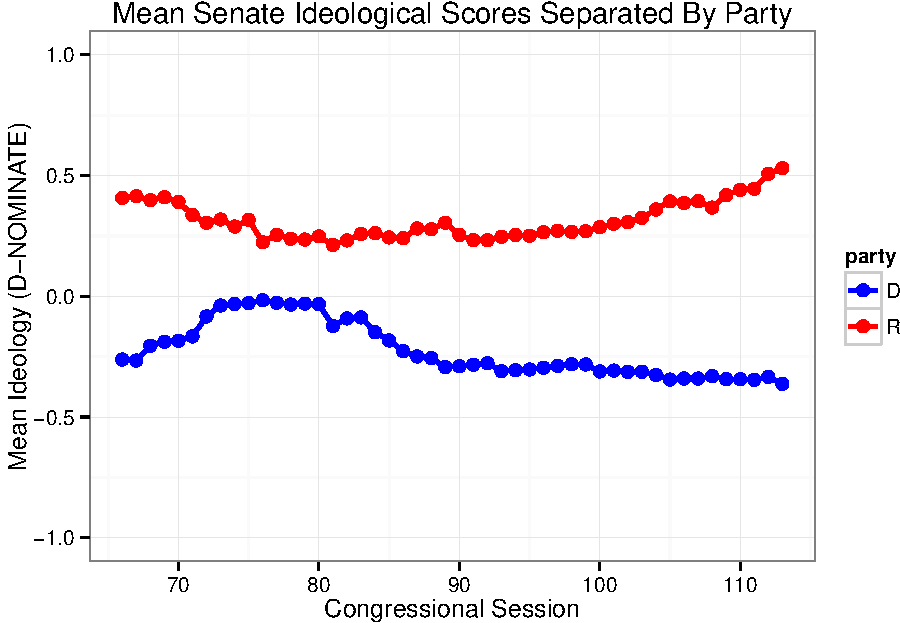
\includegraphics{trautlein_thesis_files/figure-latex/plotted_senate_means-1} \end{center}
  
  \chapter{Methodology}\label{methodology}
  
  I will use the \texttt{acf} function available in \textbf{R} to best
  estimate the number of years I should lag my data. It is assumed that I
  will see the highest correlation and covariance at the with a lag of
  \texttt{1}, meaning one congresional session behind.The correlation and
  covariance will be expected to slowly drop off. Once this \texttt{acf}
  function has been properly plotted I will be able to then move towards
  the fitting of a model to my data. To do that I will first seperate the
  data into two groups, Republicans and Democrats. Then again that data
  will be seperated into two groups, leaders and non-leaders. I will find
  the mean change of each party's ideology by congressional session within
  the \texttt{D-NOMINATE} dataset. Then I will compare the changes through
  each Congress of non-leaders to leaders within each party. This will
  allow me to see the differences in ideological change of one group
  versus the others.
  
  \chapter{Results}\label{results}
  
  Some statistically significant results are found from my regression.
  
  \begin{table}[h]
  \centering
  \caption{Summary of Models Across All Years, House and Senate}
  \begin{tabular}{r|rrrr}
                         & Senate Ds & Senate Rs & House Ds & House Rs \\ \hline
  (Intercept)            & 0.00489   & 0.00259   & 0.01131  & 0.00405  \\
  cong\_ideo\_mean       & 0.51583   & 0.61344   & 0.73047  & 0.67749  \\
  last\_cong\_ideo\_mean & -0.38112  & -0.50989  & -0.57483 & -0.53415 \\
  last\_ideo             & 0.87467   & 0.87061   & 0.87636  & 0.85013  \\
  leaderY                & \textbf{-0.01863}  & 0.01289   & -\textbf{0.03022} & -0.00417 \\
  Adjusted R-Squared     & 0.802     & 0.781     & 0.781    & 0.824    \\
  N                      & 2239      & 1817      & 11380    & 9270    
  \end{tabular}
  \end{table}
  
  These are the linear regressions computed across all the available
  congressional sessions that have complete leader data, from the 67th
  Congress to the recent 113th Congress. All of the control variables that
  were enlisted were found to be statistically signicant. These three
  variables were the idelogical mean of congress, the ideological mean of
  congress from the previous congressional session, and the
  congressperson's ideology from the previous congressional session. For
  all three of these variables across both parties in both the House and
  Senate the p-value was always less than 0.0001. It is clear that a
  legislator's current ideology would be affected by what their ideology
  was in the previous congressional session. While not as obvious, it also
  makes sense that you would need to understand the greater political
  environment that their party is in within their chamber. For example, if
  congresspeople as a whole were becoming more polarized at a rapid rate,
  as they are currently, you would expect a singular congressperson to be
  rapidly polarizing as well. Knowing how the party has changed from the
  previous congress to the most recent one allows you to help control for
  this effect.
  
  Wh
  
  .
  
  .
  
  .
  
  .
  
  .
  
  .
  
  There are five different outcomes that are possible with the above
  methodology.
  
  \begin{enumerate}
  \def\labelenumi{\arabic{enumi}.}
  \itemsep1pt\parskip0pt\parsep0pt
  \item
    A null result is found - the leaders and non-leaders do not change in
    significantly different ways.
  \item
    Leaders move to be more conservative, or right-leaning, when compared
    to non-leaders.
  \item
    Leaders move to be more liberal, or left-leaning, when compared to
    non-leaders.
  \item
    Leaders move to be more moderate, or centrist, when compared to
    non-leaders.
  \item
    Leaders move to be more extreme when compared to non-leaders.
  \end{enumerate}
  
  There are compelling reasons for many of these to be true. For outcome
  where the null result is found this could make sense if leaders and
  non-leaders have little reason to be different. One could imagine
  leaders becoming more conservative compared to non-leaders due to age of
  many of the leaders within Congress and the relation between ideology
  and age. They could become more moderate in order to fascilitate the
  dealmaking that must be done in Congress in order to get legislation
  passed. Or perhaps they would becoem more extreme in order to placate
  their more extreme bases, only choosing to delineate from them in the
  rarest of circumstances.
  
  \chapter*{Conclusion}\label{conclusion}
  \addcontentsline{toc}{chapter}{Conclusion}
  
  \setcounter{chapter}{4} \setcounter{section}{0}
  
  This study was particularly important because while a reasonable amount
  of information exists about how leaders are chosen to their positions
  based on their ideology it was not completely clear about how their
  ideology might shift after they have been selected by their fellow
  members of Congress. This thesis has looked to narrow our gap of
  understanding of these topics. However, more research is need in the
  long run especially research that involves stronger statistical methods
  that can better compensate for the sometimes small number of
  observations that exist on the models that make reference to the
  leaders. Research could also be done on whether these leaders are
  encouraging partisanship in Congress due to their ideology or halting
  it, as one of the key pieces of information found within this dataset is
  the great partisanship and polarization of the two dominating parties
  within American politics.
  
  \backmatter
  
  \chapter{Bibliography}\label{bibliography}
  
  \noindent
  
  \setlength{\parindent}{-0.20in} \setlength{\leftskip}{0.20in}
  \setlength{\parskip}{8pt}
  
  Brewer, Mark D, and Jeffrey M Stonecash. 2015. \emph{Polarization and
  the Politics of Personal Responsibility}. Oxford University Press.
  
  Clausen, Aage R, and Clyde Wilcox. 1987. ``Policy Partisanship in
  Legislative Leadership Recruitment and Behavior.'' \emph{Legislative
  Studies Quarterly}. JSTOR, 243--63.
  
  Cox, Gary W, and Mathew D McCubbins. 2005. \emph{Setting the Agenda:
  Responsible Party Government in the US House of Representatives}.
  Cambridge University Press.
  
  Dodd, Lawrence C, and Bruce I Oppenheimer. 2012. \emph{Congress
  Reconsidered}. SAGE.
  
  Evans, C Lawrence, and Walter J Oleszek. 1999. ``The Strategic Context
  of Congressional Party Leadership.'' In \emph{Congress \&Amp; the
  Presidency: A Journal of Capital Studies}, 26:1--20. 1. Taylor \&amp;
  Francis.
  
  Grofman, Bernard, William Koetzle, and Anthony J McGann. 2002.
  ``Congressional Leadership 1965--96: A New Look at the Extremism Versus
  Centrality Debate.'' \emph{Legislative Studies Quarterly} 27 (1). Wiley
  Online Library: 87--105.
  
  Harris, Douglas B, and Garrison Nelson. 2008. ``Middlemen No More?
  Emergent Patterns in Congressional Leadership Selection.'' \emph{PS:
  Political Science \&Amp; Politics} 41 (01). Cambridge Univ Press:
  49--55.
  
  Heberlig, Eric, Marc Hetherington, and Bruce Larson. 2006. ``The Price
  of Leadership: Campaign Money and the Polarization of Congressional
  Parties.'' \emph{Journal of Politics} 68 (4). Wiley Online Library:
  992--1005.
  
  Holcombe, Randall G. 2006. \emph{Public Sector Economics: The Role of
  Government in the American Economy}. Prentice Hall.
  
  Jessee, Stephen, and Neil Malhotra. 2010. ``Are Congressional Leaders
  Middlepersons or Extremists? Yes.'' \emph{Legislative Studies Quarterly}
  35 (3). Wiley Online Library: 361--92.
  
  MacDonald, Stuart Elaine, and George Rabinowitz. 1987. ``The Dynamics of
  Structural Realignment.'' \emph{American Political Science Review} 81
  (03). Cambridge Univ Press: 775--96.
  
  May, John D. 1973. ``Opinion Structure of Political Parties: The Special
  Law of Curvilinear Disparity.'' \emph{Political Studies} 21 (2). Wiley
  Online Library: 135--51.
  
  Mayhew, David R. 2004. \emph{Congress: The Electoral Connection}. 2nd
  Edition. Yale University Press.
  
  Nokken, Timothy P, and Keith T Poole. 2004. ``Congressional Party
  Defection in American History.'' \emph{Legislative Studies Quarterly} 29
  (4). Wiley Online Library: 545--68.
  
  Poole, Keith T, and Howard Rosenthal. 1991. ``Patterns of Congressional
  Voting.'' \emph{American Journal of Political Science}. JSTOR, 228--78.
  
  Poole, Keith T, and Howard L Rosenthal. 2007. \emph{Ideology and
  Congress}. Transaction Publishers.
  
  Rohde, David W. 1991. ``Parties and Leaders in the Postreform
  Congress.'' \emph{Chicago, IL: Uni}.
  
  Sinclair, Barbara, Roger H Davidson, Walter J Oleszek, Charles O Jones,
  Thomas E Mann, Norman J Ornstein, James L Sundquist, Frank H Mackaman,
  Joseph Cooper, and G Calvin Mackenzie. 1983. ``Purposive Behavior in the
  US Congress: A Review Essay.'' JSTOR.
  
  Stewart, Charles Haines. 2001. \emph{Analyzing Congress}. Norton.
  
  Theriault, Sean M. 2008. \emph{Party Polarization in Congress}.
  Cambridge University Press.


  % Index?

\end{document}

